% SC2002 --- Chapter 8: Testing & Refactoring (0->100 ground-up)
\chapter{Testing \& Refactoring: Keeping Code Correct and Clean}
\label{ch:testing}

\begin{quote}
\emph{``Refactoring without tests is not refactoring.''} --- Tests are the safety net that makes change cheap. This chapter teaches you to test behaviour (not implementation), to refactor structure while preserving behaviour, and to know when to do each.
\end{quote}

\noindent\fbox{\parbox{\dimexpr\linewidth-2\fboxsep-2\fboxrule}{%
\textbf{From zero: built on Ch.~1--7.} We define \emph{test}, \emph{oracle}, \emph{coverage}, \emph{refactor}, and \emph{code smell} from scratch. Tool: JUnit 5 + Mockito (concepts port to any framework). No prior testing assumed.}}
\vspace{0.4em}

\section*{Learning Outcomes}
After this chapter you will be able to:
\begin{enumerate}[label=(L\arabic*)]
    \item write JUnit 5 tests (arrange--act--assert), use fixtures, and distinguish unit vs.\ integration tests;
    \item apply equivalence partitioning and boundary-value analysis to choose minimal, high-yield test cases;
    \item use test doubles (stub, mock, spy) and explain when to mock and when not to;
    \item refactor safely via small, behaviour-preserving steps (extract method/class, replace conditional with polymorphism, etc.);
    \item measure and interpret coverage without gaming it, and run a TDD red--green--refactor cycle.
\end{enumerate}

% ============================================================
\section{Testing: The Safety Net}
\label{sec:testing}
Tests \emph{specify} expected behaviour and \emph{detect} regressions. A good test is fast, isolated (no shared mutable state), and asserts on observable behaviour, not internal wiring.

\begin{lstlisting}[language=Java, caption={JUnit 5 basics---arrange, act, assert; fixture with BeforeEach.}]
import static org.junit.jupiter.api.Assertions.*;
import org.junit.jupiter.api.*;

class BookTest {
    private Book book;
    @BeforeEach void setUp(){ book = new Book("Dune"); } // fixture
    @Test void newBookIsAvailable(){ assertTrue(book.isAvailable()); }
    @Test void borrowMakesUnavailable(){
        book.markBorrowed();
        assertFalse(book.isAvailable());
    }
    @Test void doubleBorrowThrows(){
        book.markBorrowed();
        assertThrows(IllegalStateException.class, () -> book.markBorrowed());
    }
    @Test @DisplayName("toString contains title") void toStringHasTitle(){
        assertTrue(book.toString().contains("Dune"));
    }
}
\end{lstlisting}

% --- TikZ 1: AAA + test pyramid ---
\begin{figure}[h]
\centering
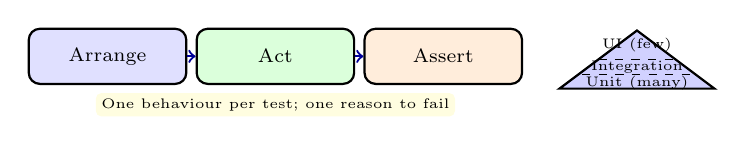
\begin{tikzpicture}[scale=0.82, every node/.style={font=\scriptsize}]
% AAA blocks
\node[draw,thick,fill=blue!12,rounded corners=4pt,minimum width=2.0cm,minimum height=0.7cm] (arr) at (0,0.6) {Arrange};
\node[draw,thick,fill=green!14,rounded corners=4pt,minimum width=2.0cm,minimum height=0.7cm] (act) at (2.6,0.6) {Act};
\node[draw,thick,fill=orange!14,rounded corners=4pt,minimum width=2.0cm,minimum height=0.7cm] (ass) at (5.2,0.6) {Assert};
\draw[->,thick,blue!60!black] (arr) -- (act);
\draw[->,thick,blue!60!black] (act) -- (ass);
\node[font=\tiny,fill=yellow!12,rounded corners=2pt,inner sep=2pt] at (2.6,-0.15) {One behaviour per test; one reason to fail};
% Pyramid
\begin{scope}[xshift=8.2cm, yshift=0.1cm]
\fill[blue!18] (0,0.9) -- (1.2,0) -- (-1.2,0) -- cycle;
\draw[thick] (0,0.9) -- (1.2,0) -- (-1.2,0) -- cycle;
\draw[dashed] (-0.6,0.45) -- (0.6,0.45);
\draw[dashed] (-0.85,0.22) -- (0.85,0.22);
\node[font=\tiny] at (0,0.68) {UI (few)};
\node[font=\tiny] at (0,0.33) {Integration};
\node[font=\tiny] at (0,0.08) {Unit (many)};
\end{scope}
\end{tikzpicture}
\caption{Left: Arrange--Act--Assert (one behaviour per test). Right: test pyramid---many fast unit tests, fewer integration/UI tests.}
\label{fig:aaa-pyramid}
\end{figure}

\paragraph{Choosing test cases.} No exhaustive testing. Use \emph{equivalence partitions} (inputs that should behave the same) and \emph{boundary values} (edges: 0, 1, MAX, null, empty). For \texttt{canBorrow} with limit 5: test 0, 4, 5, 6 loans; for \texttt{dueDate}: on-time, one day late, far overdue.

\paragraph{Test doubles.} When a unit depends on slow/fragile collaborators (DB, network), replace them: \emph{stub} (returns canned data), \emph{mock} (verifies interactions), \emph{spy} (wraps real object), \emph{fake} (lightweight working implementation). Mock only across boundaries you own---over-mocking couples tests to implementation.

\begin{lstlisting}[language=Java, caption={Mocking a collaborator---verify interaction, not just state.}]
import static org.mockito.Mockito.*;

class CheckoutTest {
    @Test void borrowDelegatesToBook(){
        Book mockBook = mock(Book.class);
        when(mockBook.isAvailable()).thenReturn(true);
        Member m = new Member("u1", 5);
        Loan loan = Loan.create(m, mockBook);
        verify(mockBook).markBorrowed(); // interaction asserted
        assertNotNull(loan);
    }
}
\end{lstlisting}

% --- TikZ 2: Coverage vs confidence ---
\begin{figure}[h]
\centering
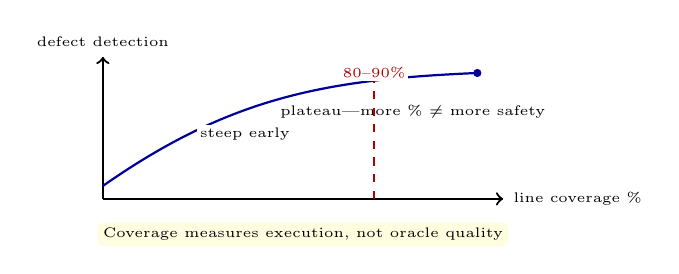
\begin{tikzpicture}[scale=0.82, every node/.style={font=\scriptsize}]
\draw[->,thick] (0,0) -- (6.2,0) node[right,font=\tiny] {line coverage \%};
\draw[->,thick] (0,0) -- (0,2.2) node[above,font=\tiny] {defect detection};
\draw[thick,blue!60!black] (0,0.2) .. controls (2.0,1.6) and (3.5,1.85) .. (5.8,1.95);
\fill[blue!60!black] (5.8,1.95) circle (1.8pt);
\node[font=\tiny,fill=white,inner sep=1pt] at (2.2,1.0) {steep early};
\node[font=\tiny,fill=white,inner sep=1pt] at (4.8,1.35) {plateau---more \% $\neq$ more safety};
\draw[dashed,red!70!black] (4.2,0) -- (4.2,1.82) node[above,font=\tiny,fill=white,inner sep=1pt] {80--90\%};
\node[font=\tiny,align=center,fill=yellow!12,rounded corners=2pt,inner sep=2pt] at (3.1,-0.55) {Coverage measures execution, not oracle quality};
\end{tikzpicture}
\caption{Coverage vs.\ confidence: early coverage finds real gaps; chasing 100\% often tests trivial code while missing semantics.}
\label{fig:coverage-confidence}
\end{figure}

\section{Refactoring: Change Structure, Preserve Behaviour}
\label{sec:refactoring}
A \emph{refactor} is a behaviour-preserving transformation that improves structure (readability, cohesion, coupling). Refactors are small and sequenced; tests stay green after each step. Big-bang rewrites are not refactors.

\begin{figure}[h]
\centering
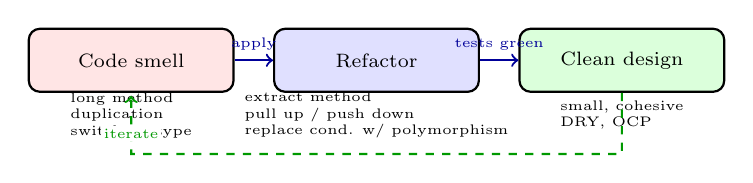
\begin{tikzpicture}[scale=0.82, every node/.style={font=\scriptsize}]
\node[draw,thick,fill=red!10,rounded corners=4pt,minimum width=2.6cm,minimum height=0.8cm] (smell) at (0,0) {Code smell};
\node[draw,thick,fill=blue!12,rounded corners=4pt,minimum width=2.6cm,minimum height=0.8cm] (ref) at (3.8,0) {Refactor};
\node[draw,thick,fill=green!14,rounded corners=4pt,minimum width=2.6cm,minimum height=0.8cm] (clean) at (7.6,0) {Clean design};
\draw[->,thick,blue!60!black] (smell) -- (ref) node[midway,above,font=\tiny] {apply};
\draw[->,thick,blue!60!black] (ref) -- (clean) node[midway,above,font=\tiny] {tests green};
\node[font=\tiny,align=left] at (0,-0.85) {long method\\duplication\\switch on type};
\node[font=\tiny,align=left] at (3.8,-0.85) {extract method\\pull up / push down\\replace cond. w/ polymorphism};
\node[font=\tiny,align=left] at (7.6,-0.85) {small, cohesive\\DRY, OCP};
\draw[->,thick,green!60!black,dashed] (clean) -- (7.6,-1.45) -- (0,-1.45) -- (0,-0.55) node[midway,below,font=\tiny,fill=white,inner sep=1pt] {iterate};
\end{tikzpicture}
\caption{Refactoring loop: detect a smell, apply a small behaviour-preserving refactor, verify with tests, repeat.}
\label{fig:refactor-loop}
\end{figure}

Common refactors and the smells they cure:
\begin{itemize}[itemsep=0.25em]
    \item \emph{Extract Method/Class} $\gets$ long method / god class (SRP).
    \item \emph{Replace Conditional with Polymorphism} $\gets$ switch-on-type (OCP)---introduce Strategy/hierarchy from Ch.~6.
    \item \emph{Move Method} $\gets$ feature envy (method uses another class's data more than its own).
    \item \emph{Introduce Parameter Object / Builder} $\gets$ long parameter list.
\end{itemize}

\begin{lstlisting}[language=Java, caption={Refactor: replace switch with polymorphism (Ch.~5--6 applied).}]
// Before: violates OCP, hard to test
double shippingCost(String type, double w){
    switch(type){ case "standard": return 5+0.5*w; case "express": return 12+1.2*w; default: throw new IllegalArgumentException(); }
}
// After: each variant is a class; adding a variant touches no existing class
interface ShippingStrategy{ double cost(double w); }
class StandardShipping implements ShippingStrategy{ public double cost(double w){return 5+0.5*w;}}
class ExpressShipping  implements ShippingStrategy{ public double cost(double w){return 12+1.2*w;}}
// Client now depends on abstraction (DIP), tests inject a stub strategy
\end{lstlisting}

\subsection{TDD: Red--Green--Refactor}
\emph{Test-Driven Development} inverts the order: write a failing test (red), write minimal code to pass (green), refactor with safety. Benefits: tests actually get written, design stays testable, scope stays minimal. Trade-off: not suited for exploratory spikes where the interface is unknown.

\begin{remark}[Coverage guidance]
Aim for high coverage on domain logic; do not chase 100\% by testing getters/setters. Mutation testing (PIT) is a stronger signal: it checks whether tests \emph{detect} injected faults, not just execute lines.
\end{remark}

\section{Refactoring Catalogue in Detail}
\label{sec:refactoring-catalogue}
Each refactor below is a small, named, behaviour-preserving step. Apply one at a time and run tests after each.

\paragraph{Extract Method.} Long method with a coherent chunk $\to$ new private method with a descriptive name. Improves readability and enables reuse. Precondition: extracted code has no hidden side-effects on local control flow.

\paragraph{Extract Class / Move Method.} Method on \texttt{A} that uses \texttt{B}'s data more than \texttt{A}'s $\to$ move it to \texttt{B} (feature envy). Class with two axes of change $\to$ split into two classes (SRP).

\paragraph{Replace Conditional with Polymorphism.} Switch/if-chain on type tag $\to$ introduce a Strategy/hierarchy (Ch.~6). OCP payoff: new variants add classes, not edits.

\paragraph{Introduce Parameter Object / Builder.} Method with 4+ parameters or telescoping constructors $\to$ bundle into a parameter object or Builder. Reduces call-site errors and documents the parameter set.

\begin{lstlisting}[language=Java, caption={Introduce Parameter Object + Builder for a telescoping constructor.}]
// Before: confusing, error-prone call
Loan l = new Loan(member, book, dueDate, true, false, null);
// After: self-documenting, validated at build time
Loan l2 = Loan.builder().borrower(member).book(book).dueDate(dueDate).build();
\end{lstlisting}

\subsection{TDD Traces and When Not to Mock}
TDD trace for \texttt{Money}: (1) red: \texttt{Money.of(10,"SGD").plus(Money.of(5,"SGD")) == Money.of(15,"SGD")}; (2) green: naive add; (3) refactor: handle currency mismatch $\to$ throw. Each cycle is minutes, not hours.

Mock sparingly: mock I/O boundaries (repository, gateway), not value objects (\texttt{Money}, \texttt{Isbn}) or stable domain entities. Over-mocking makes tests brittle to internal renames.

\begin{remark}[Safe refactoring checklist]
Before refactoring: green tests, small commit. During: one refactor per commit, no behaviour change. After: tests still green, review for accidental semantics change (especially around equals/hashCode and exception paths).
\end{remark}

\section{Chapter Notes}
Refactoring catalogue is Fowler (1999/2018); TDD is Beck (2002). JUnit 5 User Guide and Mockito docs are the practical references. Coverage vs.\ mutation is discussed in Effective Software Testing (Maurer \& Scheffczyk). Clean Code (Martin) covers smell naming.

\section{Exercises}
\label{sec:ch08-exercises}
\begin{enumerate}[label=E8.\arabic*, leftmargin=*, itemsep=0.8em]
    \item \textbf{AAA audit.} A test has 30 lines, 4 assertions, and touches DB + filesystem. Diagnose using AAA, isolation, and pyramid guidance, then split it into focused unit tests with fakes/mocks.
    \item \textbf{Partitions \& boundaries.} For ``loan period 14 days, fine \$1/day after 7-day grace, max fine \$30,'' list equivalence partitions and boundary values. Write the minimal JUnit cases that cover them.
    \item \textbf{Mock boundary.} \texttt{Checkout.borrow} calls \texttt{Book.isAvailable()} and \texttt{Member.canBorrow()}. Which collaborators should be mocked in a unit test of \texttt{Checkout} and which should be real? Justify with coupling and oracle strength.
    \item \textbf{Refactor sequence.} Apply ``Replace Conditional with Polymorphism'' to the shipping-cost switch in the listing. List the steps in order (create interface, extract strategies, update client, run tests) and state what could go wrong if done as one big edit.
    \item \textbf{TDD cycle.} Using TDD, implement \texttt{Money} (immutable, currency-aware, add/subtract with same currency, no floating point). Show the red--green--refactor sequence for the first three tests and the design decisions each forced.
\end{enumerate}
% End of Chapter 8
